\section{Wahrscheinlichkeit und Statistik}

\subsection{Zufallsexperiment}
\begin{tabular}{|l|l|}
	\hline
	Experiment & Beobachtungsprozess, Ergebnis anschliessend ausgewertet. Ergebnis zuvor unbestimmt\\
	\hline
	Elementarereignis ($\lambda$) & Einzelne Resultate des Experiments\\
	\hline
	Ereignis & Einzelne Versuchsausgänge zusammengefasst (Beispiel Gerade Zahlen)\\
	\hline
	Ergebnisraum ($S$) & Alle möglichen Versuchsausgänge\\
	\hline
	Disjunkt & Ereignisse sind disjunkt, wenn sie keine gemeinsame Elemente beinhalten.\\
	\hline
\end{tabular}

\subsection{Verknüpfung von Ereignissen}

\begin{minipage}[t]{0.85\textwidth}
	%{m{2cm}m{1cm}c} {|l|l|c|c|}
	\begin{tabular}[t]{|m{3.4cm}|m{4.5cm}|m{2.5cm}|m{1.8cm}|}
		\hline
		Begriff & Beschreibung & Bild & Modell\\
		\hline
		Sicheres Ereignis & tritt immer ein & %Autor: Simon Walker
%Version: 1.5
%Datum: 06.07.2020
%Lizenz: CC BY-NC-SA
%Quelle WarStat ZF HS19 https://github.com/RostBau/WrStat oder https://github.com/HSR-Stud/WrStat

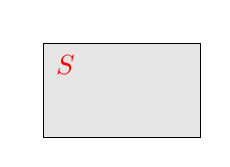
\begin{tikzpicture}[xscale=0.4, yscale=0.4]
	\fill[white, fill opacity=0] (-0.5,0) rectangle (5, 3.5); % Weisser rand um Grafik
	
	\fill[gray!20] (0,0) rectangle (5,3);
	\draw (0,0) rectangle (5,3);
	\node[red] at (0.7,2.3) {$S$};
	
	%\draw[help lines] (0,0) grid (5,3);
\end{tikzpicture}
 & $S$\\
		\hline
		Unmögliches Ereignis & kann nicht eintreten & %Autor: Simon Walker
%Version: 1.5
%Datum: 06.07.2020
%Lizenz: CC BY-NC-SA
%Quelle WarStat ZF HS19 https://github.com/RostBau/WrStat oder https://github.com/HSR-Stud/WrStat

\begin{tikzpicture}[xscale=0.4, yscale=0.4]
	\fill[white, fill opacity=0] (-0.5,0) rectangle (5, 3.5); % Weisser rand um Grafik
	
	\fill[white] (0,0) rectangle (5,3);
	\draw (0,0) rectangle (5,3);
	\node[red] at (0.7,2.3) {$S$};
	
	%\draw[help lines] (0,0) grid (5,3);
\end{tikzpicture}
 & $\emptyset = \{\}$\\
		\hline
		Disjunkte Ereignisse & Keine gemeinsame Elemente & %Autor: Simon Walker
%Version: 1.0
%Datum: 06.07.2020
%Lizenz: CC BY-NC-SA

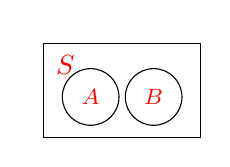
\begin{tikzpicture}[xscale=0.4, yscale=0.4]
	\fill[white, fill opacity=0] (-0.5,0) rectangle (5, 3.5); % Weisser rand um Grafik
	
	\draw (0,0) rectangle (5,3);
	\node[red] at (0.7,2.3) {$S$};
	
	\draw (1.5,1.3) circle[radius=0.9];
	\draw (3.5,1.3) circle[radius=0.9];
	
	
	\node[red] at (1.5, 1.3) {\footnotesize$A$};
	\node[red] at (3.5, 1.3) {\footnotesize$B$};
	
	%\draw[help lines] (0,0) grid (5,3);
\end{tikzpicture}
 & $A \cap B = \emptyset$\\
		\hline
		$A$ und $B$ & Schnittmenge & %Autor: Simon Walker
%Version: 1.5
%Datum: 06.07.2020
%Lizenz: CC BY-NC-SA
%Quelle WarStat ZF HS19 https://github.com/RostBau/WrStat oder https://github.com/HSR-Stud/WrStat

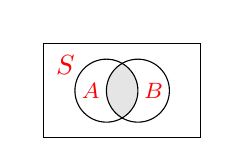
\begin{tikzpicture}[xscale=0.4, yscale=0.4]
	\fill[white, fill opacity=0] (-0.5,0) rectangle (5, 3.5); % Weisser rand um Grafik
	
	
	%\fill[white] (0,0) rectangle (5,3);
	\draw (0,0) rectangle (5,3);
	\node[red] at (0.7,2.3) {$S$};
	
	\begin{scope} %Schnittmenge färben
		\clip (2,1.5) circle[radius=1];
		\fill[gray!20] (3,1.5) circle[radius=1];
	\end{scope}
	
	\draw (2,1.5) circle[radius=1]; %Kreise Zeichnen
	\draw (3,1.5) circle[radius=1];
	
	\node[red] at (1.5, 1.5) {\footnotesize$A$};
	\node[red] at (3.5, 1.5) {\footnotesize$B$};
	
	%\draw[help lines] (0,0) grid (5,3);
\end{tikzpicture}
 & $A \cap B$\\
		\hline
		$A$ oder $B$ & Vereinigung & %Autor: Simon Walker
%Version: 1.5
%Datum: 06.07.2020
%Lizenz: CC BY-NC-SA
%Quelle WarStat ZF HS19 https://github.com/RostBau/WrStat oder https://github.com/HSR-Stud/WrStat

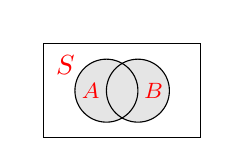
\begin{tikzpicture}[xscale=0.4, yscale=0.4]
	\fill[white, fill opacity=0] (-0.5,0) rectangle (5, 3.5); % Weisser rand um Grafik
	
	%\fill[white] (0,0) rectangle (5,3);
	\draw (0,0) rectangle (5,3);
	\node[red] at (0.7,2.3) {$S$};
	
	\fill[gray!20] (2,1.5) circle[radius=1]; %Fläche färben
	\fill[gray!20] (3,1.5) circle[radius=1];
	
	\draw (2,1.5) circle[radius=1]; %Kreise Zeichnen
	\draw (3,1.5) circle[radius=1];
	
	\node[red] at (1.5, 1.5) {\footnotesize$A$};
	\node[red] at (3.5, 1.5) {\footnotesize$B$};
	
	%\draw[help lines] (0,0) grid (5,3);
\end{tikzpicture}
 & $A \cup B$\\
		\hline
		$A$ hat $B$ zur folge & A ist in B enthalten & %Autor: Simon Walker
%Version: 1.5
%Datum: 06.07.2020
%Lizenz: CC BY-NC-SA
%Quelle WarStat ZF HS19 https://github.com/RostBau/WrStat oder https://github.com/HSR-Stud/WrStat

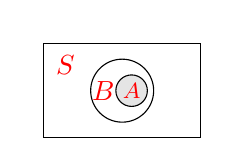
\begin{tikzpicture}[xscale=0.4, yscale=0.4]
	\fill[white, fill opacity=0] (-0.5,0) rectangle (5, 3.5); % Weisser rand um Grafik
	
	%\fill[white] (0,0) rectangle (5,3);
	\draw (0,0) rectangle (5,3);
	\node[red] at (0.7,2.3) {$S$};
	
	\fill[white] (2.5, 1.5) circle [radius=1];
	\draw (2.5,1.5) circle [radius=1];
	\node[red] at (1.9, 1.5) {$B$};
	
	\fill[gray!20] (2.8, 1.5) circle [radius=0.5];
	\draw (2.8,1.5) circle [radius=0.5];
	\node[red] at (2.8, 1.5) {\footnotesize $A$};
	
	
	%\draw[help lines] (0,0) grid (5,3);
\end{tikzpicture}
 & $A \subset B$ \\
		\hline
		nicht $A$ & Komplementär Ereignis & %Autor: Simon Walker
%Version: 1.5
%Datum: 06.07.2020
%Lizenz: CC BY-NC-SA
%Quelle WarStat ZF HS19 https://github.com/RostBau/WrStat oder https://github.com/HSR-Stud/WrStat

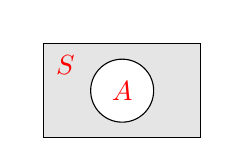
\begin{tikzpicture}[xscale=0.4, yscale=0.4]
	\fill[white, fill opacity=0] (-0.5,0) rectangle (5, 3.5); % Weisser rand um Grafik
		
	\fill[gray!20] (0,0) rectangle (5,3);
	\draw (0,0) rectangle (5,3);
	\node[red] at (0.7,2.3) {$S$};
	
	\fill[white] (2.5, 1.5) circle [radius=1];
	\draw (2.5,1.5) circle [radius=1];
	
	\node[red] at (2.5, 1.5) {$A$};
	
	%\draw[help lines] (0,0) grid (5,3);
\end{tikzpicture}
 & $\bar{A} = S\setminus A$\\
		\hline
	\end{tabular}
\end{minipage} %
\begin{minipage}[t]{0.15\textwidth}
	\vspace{10pt}
	$\bar{S} = \emptyset$\\
	$\bar{\emptyset} = S$\\
	$S \cup A = S$\\
	$S \cap A = A$\\
	$A \cup \bar{A} = S$\\
	$A \cap \bar{A} = S$\\
	$\bar{\bar{A}} = A$\\
\end{minipage}

\subsection{Wahrscheinlichkeit von Ereignissen}
\begin{minipage}{0.7\textwidth}
	Bei der Wahrscheinlichkeit von Ereignissen handelt sich um eine Funktion $P(A)$ welche jedem Ereignis $A \subset S$ eine reelle Zahl zuweist.
\end{minipage}
\begin{minipage}{0.3\textwidth}
	\begin{center}
		\fbox{$P(A) = \lim\limits_{n\rightarrow \infty} \dfrac{n_A}{n}$}
	\end{center}
\end{minipage}

\subsubsection{Axiomen}
\begin{minipage}[t]{0.32\textwidth}
	$P(A)\ge 0$\\
	$P(S) = 1$\\[4pt]
	falls $A$ und $B$ disjunkt\\
	$P(A \cup B) = P(A) + P(B)$ 
\end{minipage}
\begin{minipage}[t]{0.32\textwidth}
	$P(\bar{A}) = 1 - P(A)$\\
	$P(\emptyset) = 0$\\
	$B \subset A \rightarrow P(B) \le P(A)$
\end{minipage}
\begin{minipage}[t]{0.35\textwidth}
	$P(A) \le 1$\\[4pt]
	falls $A$ und $B$ nicht disjunkt\\
	$P(A \cup B) = P(A) + P(B) - P(A \cap B)$ 
\end{minipage}

\subsubsection{Laplace-Experiment}
\begin{multicols}{2}
	Ein Laplace-Experiment ist ein Zufallsexperiment bei welchem die endliche Anzahl von mögliche Ausgänge alle gleich häufig vorkommen.\\
	\columnbreak
	\begin{center}
		\fbox{$P(\lambda_i) = \dfrac{1}{n}$ \quad für alle $1 \le i \le n$}
	\end{center}
\end{multicols}


\subsubsection{Bedingte Wahrscheinlichkeit}
\begin{multicols}{2}
	\fbox{$ P(B|A) = \dfrac{P(B \cap A)}{P(A)} $} $=\underbrace{\frac{P(A) \cdot P(B)}{P(B)}=P(A)}_{\text{nur wenn unabhängig}}$
	\columnbreak\\
	$P(B|A)$ ist die Wahrscheinlichkeit das ein das Ereignis $B$ eintritt unter der Voraussetzung das $A$ bereits eingetroffen ist.
\end{multicols}

\subsubsection{Satz von Bayes}
\begin{minipage}{0.58\textwidth}
Tauscht die Ereignisse der Bedingten Wahrscheinlichkeit.
\end{minipage}
\hspace{0.04\textwidth}
\begin{minipage}{0.38\textwidth}
	\begin{center}
		\fbox{$P(B \mid A)=P(A \mid B) \cdot \dfrac{P(B)}{P(A)}$}
	\end{center}
\end{minipage}

\subsubsection{Unabhängige Ereignisse}
Für sie gilt: \fbox{$P(A \cap B)=P(A) P(B)$}\\[5pt]
Die Tatsache, dass $A$ eingetreten ist, hat keinen Einfluss auf die Wahrscheinlichkeit von $B$.\\
Wenn Ereignisse nicht gleichzeitig eintreten können, so sind sie abhängig.

\subsubsection{Satz von der totalen Wahrscheinlichkeit}
\fbox{$\displaystyle P(A)=\sum_{i=1}^{n} P(A | B_i) \cdot P(B_i)$} \qquad
Die Ereignisse $B_i$ müssen disjunkt sein.

\subsection{Zufallsvariable}
Eine Zufallsvariable $X(\lambda)$ ist eine Funktion die jedem Ergebnis $\lambda_i$ eine reelle Zahl zuweist.

\subsubsection{Zweidimensionale Zufallsvariable}
Die zwei Zufallsvariablen $X(\lambda)$ und $Y(\lambda)$ weisen jedem Ergebnis $\lambda_i$ des Ergebnisraums $S$ zwei reelle Zahlen zu. Diese zwei Zufallsvariablen können voneinander abhängig oder unabhängig sein.
Bsp: Prüfungsnote und Erfolgserlebnis der Studenten.

\subsubsection{Verteilungsfunktion}
Die Verteilungsfunktion $F_X(x)$ gibt an, welcher statistische Anteil von Ergebnissen der Zufallsvariable $X(\lambda)$ einen kleineren Wert als $x$ aufweist.
\begin{center}
	\fbox{$F_X(x) = P(X \le x)$} \qquad für $-\infty < x < \infty$
\end{center}

\textbf{Eigenschaften:}
\begin{multicols}{2}
	$0 \le F_X(x) \le 1$\\
	$F_X(x_1) \le F_X(x_2)$ für $x_1 < x_2$
	\columnbreak\\
	$F_X(-\infty) = 0$\\
	$F_X(+\infty) = 1$
\end{multicols}

\subsubsection{Wahrscheinlichkeitsdichtefunktion}
\begin{minipage}[t]{0.48\textwidth}
	\textbf{Stetige Zufallsvariable:}\\
	Die Dichtefunktion für eine Stetige Zufallsvariable ist die Ableitung der Verteilungsfunktion $F_X(x)$.
	\begin{center}
		\fbox{$f_X(x)=\dfrac{dF_X(x)}{dx}$}
	\end{center}
\textbf{Eigenschaften:}\\
$f_X(x)$ ist stückweise Stetig\\
$f_X(x) \ge 0$\\
$\int\limits_{-\infty}^{\infty} f_X(x) dx = 1$\\
$P(a < X \le b) = \int\limits_{a^+}^{b} f_X(x) dx$
\end{minipage} \hspace{0.04\textwidth}
\begin{minipage}[t]{0.48\textwidth}
	\textbf{Diskrete Zufallsvariable:}\\
	Die Verteilungsfunktion $F_X(x)$ von diskreten Zufallsvariablen weist Sprungstellen auf für diese Stellen existiert dann keine Ableitung. Dieses Problem wird mit Dirac-Implusen welche gerade mit der Sprunghöhe von $F_X(x)$ gewichtet wird.
	\begin{center}
		\fbox{$f_X(x) = \sum\limits_{1}^{n} (F_X(x_{i+1}) - F_X(x_i)) \cdot \delta(x-x_i)$}
	\end{center}
\end{minipage}

\subsubsection{Erwartungswert}
Der Erwartungswert $\mu_X$ gibt den Mittelwert der Zufallsvariable $X(\lambda)$ wieder wobei die Werte $X(\lambda) = x$ mit den Auftretungswahrscheinlichkeit $p_X(x) = P(X=x)$ gewichtet werden.\\[3pt]
\begin{minipage}[t]{0.48\textwidth}
	\textbf{Diskret}\\
	\fbox{$\mu_X = E[X] = \sum\limits_{i}^{\quad}x_i \cdot p_X(x_i)$}
\end{minipage} \hspace{0.04\textwidth}
\begin{minipage}[t]{0.48\textwidth}
	\textbf{Stetig}\\
	\fbox{$\mu_X = E[X] = \int\limits_{-\infty}^{\infty} x \cdot f_X(x) \: dx$}
\end{minipage}

\subsubsection{Zweites und n-tes Moment}
\begin{minipage}[t]{0.48\textwidth}
	\textbf{Diskret}\\
	\fbox{$E[X^2] = \sum\limits_{i}^{\quad}{x_i}^2 \cdot p_X(x_i)$}\\[3pt]
	$E[X^n] = \sum\limits_{i}^{\quad}{x_i}^n \cdot p_X(x_i)$
\end{minipage} \hspace{0.04\textwidth}
\begin{minipage}[t]{0.48\textwidth}
	\textbf{Stetig}\\
	\fbox{$E[X^2] = \int\limits_{-\infty}^{\infty} x^2 \cdot f_X(x) \: dx$}\\[3pt]
	$E[X^n] = \int\limits_{-\infty}^{\infty} x^n \cdot f_X(x) \: dx$
\end{minipage}

\subsubsection{Varianz und Standartabweichung}
Bei der Varianz handelt es sich um ein statistisches Leistungsmass, welche die mittlere Abweichung vom Erwartungswert ausdrückt.\\[3pt]
\fbox{$\sigma^2 = Var[X] = E[(X-\mu_X)^2]$}\\[5pt]
\begin{minipage}[t]{0.48\textwidth}
	\textbf{Diskret}\\
	$Var[X] = \sum\limits_{i}^{\,} (x_i -\mu_X)^2 \cdot p_X(x_i)$\\
\end{minipage} \hspace{0.04\textwidth}
\begin{minipage}[t]{0.48\textwidth}
	\textbf{Stetig}\\
	$Var[X] = \int\limits_{-\infty}^{\infty} (x -\mu_X)^2 \cdot f_X(x) \: dx$
\end{minipage}
\textbf{Standartabweichung:}\\
\fbox{$\sigma = \sqrt{Var[X]}$}

\subsubsection{Korrelation}
Korrelation ist ein statistische Kennwert zweier Zufallsvariablen $X$ und $Y$, welcher einen allfälligen linearen Zusammenhang ausdrückt. Die Korrelation ist eine statistische Kreuzleistung.\\
\begin{minipage}[t]{0.48\textwidth}
	\textbf{Diskret}\\
	\fbox{$m_{11} = E[X \cdot Y] = \sum\limits_{i}^{\quad}\sum\limits_{k}^{\quad}x_i\cdot y_k \cdot p_{XY}(x_i, y_k)$}\\
\end{minipage} \hspace{0.04\textwidth}
\begin{minipage}[t]{0.48\textwidth}
	\textbf{Stetig}\\
	\fbox{$m_{11} = E[X \cdot Y] = \int\limits_{-\infty}^{\infty}\int\limits_{-\infty}^{\infty} x\cdot y \cdot f_XY(x, y) \: dx \: dy$}
\end{minipage}
\textbf{Eigenschaften:}\\
Zwei Zufallsvariablen $X$ und $Y$ sind zueinander orthogonal falls $m_{11} = 0$ ist\\
Wenn $X$ und $Y$ beide Mehrheitlich das gleiche Vorzeichen haben, dann ist $m_{11}$ positiv. Ist das Vorzeichen mehrheitlich verschieden, dann ist $m_{11}$ negativ.
 
\subsubsection{Kovarianz}
Die Kovarianz ist grundsätzlich das selbe wie bei der Korrelation. Nur werden die Zufallszahlen durch ihren Erwartungswert bereinigt\\
\fbox{$\sigma_{XY} = E[(X-\mu_X) \cdot (Y-\mu_Y)]$}\\[5pt]
\begin{minipage}[t]{0.48\textwidth}
	\textbf{Diskret}\\
	$\sigma_{XY} = \sum\limits_{k}\sum\limits_{i} (x_i-\mu_X)\cdot (y_K - \mu_Y)\cdot p_{XY}(x_i,y_k)$
\end{minipage} \hspace{0.04\textwidth}
\begin{minipage}[t]{0.48\textwidth}
	\textbf{Stetig}\\
	$\sigma_{XY} = \int\limits_{-\infty}^{\infty}\int\limits_{-\infty}^{\infty} (x-\mu_X)\cdot (y - \mu_Y)\cdot f_{XY}(x,y) \: dx \: dy$
\end{minipage}

\subsection{Wahrscheinlichkeitsverteilung}
\subsubsection{Gleichverteilung}
\begin{minipage}[t]{0.48\textwidth}
	\textbf{Diskret}\\
	\fbox{$p_X(x_i) = \dfrac{1}{n}$}\\[3pt]
	
\end{minipage} \hspace{0.04\textwidth}
\begin{minipage}[t]{0.3\textwidth}
	\textbf{Stetig}\\
	\fbox{$f_X(x) = \dfrac{1}{b-a}$}
\end{minipage}

\subsubsection{Binomialverteilung}
Wird angewendet bei einem Experiment mit nur zwei Ausgängen (Ereignis mit Wahrscheinlichkeit $p$ tritt ein, Ereignis tritt nicht ein) zu beschreiben. Die Binomialverteilung gibt an wie Wahrscheindlich es ist, mit $n$ Versuche $k$-mal erfolgreich zu sein. \\
\vrule \begin{minipage}{0.41\textwidth}
	\hrule
	\vspace{5pt}
	\leftskip8pt $p_X(k)=P(X=k)=\left(\begin{array}{l}
	n \\
	k
	\end{array}\right) p^{k}(1-p)^{n-k}$\\
	$\mu_X=n \cdot p$\\
	$\sigma^{2}=\operatorname{var}(X)=n \cdot p(1-p)$
	\vspace{5pt}
	\hrule
\end{minipage}\vrule \hspace{0.04\textwidth}
\begin{minipage}{0.55\textwidth}
	$n$: Versuche \quad $k$: k-mal erfolgreich \quad $p$: Wahrscheinlichkeit
\end{minipage}\\[5pt]
\color{red} \textbf{Achtung!:} \color{black} Für seltene Ereignisse Poissonverteilung verwenden!

\subsubsection{Poissonverteilung}
Die Poissonverteilung entspricht der Binomialverteilung für seltene Ereignisse ($n$ sehr gross und die Wahrscheinlichkeit $p$ sehr klein).\\
\fbox{$p_X(k) = P(X=k) = e^{-n\cdot p} \cdot \dfrac{(n\cdot p)^k}{k!}$} \qquad $E(X)=\mu_X = n \cdot p$ \qquad $var(X)=\sigma^2 = n \cdot p$

\subsubsection{Gaussverteilung}
Gaussverteilung oder Normalverteilung\\
\fbox{$f_X(x)=\dfrac{1}{\sqrt{2 \pi}\cdot \sigma}e^{\frac{-(x-\mu)^2}{2\sigma^2}}$}\\
Die Verteilungsfunktion $F(x)=\frac{1}{\sqrt{2 \pi} \sigma} \cdot \int_{-\infty}^{x} e^{-\frac{(\tilde{x}-\mu)^{2}}{2 \sigma^{2}}} d \tilde{x}$ lässt sich nicht analytisch berechnen. Deshalb muss dies numerisch über Tabellen ausgelesen werden.\\
In Nat2 wird dies über die Fehlerfunktion oder über die Q-Funktion gelöst (siehe Skript Nat1\&2 s137-140)\\
Ansonsten muss die Verteilung standardisiert werden $\sigma^2 = 1$ \& $\mu = 0$. Dies geschieht mit folgender Formel: $\frac{x-\mu}{\sigma}$\\
Danach kann man den Wert aus der Tabelle auslesen\\
\subsubsection{Verteilungsfunktion der Normalverteilung}
	\label{tbl_NormVerteilung}

\begin{tabular}{|r|rrrrrrrrrr|}
	\hline
	$x$&+0.00&+0.01&+0.02&+0.03&+0.04&+0.05&+0.06&+0.07&+0.08&+0.09\\
	\hline
	\rowcolor[gray]{.9}
	0.0&0.5000&0.5040&0.5080&0.5120&0.5160&0.5199&0.5239&0.5279&0.5319&0.5359\\
	0.1&0.5398&0.5438&0.5478&0.5517&0.5557&0.5596&0.5636&0.5675&0.5714&0.5753\\
	\rowcolor[gray]{.9}
	0.2&0.5793&0.5832&0.5871&0.5910&0.5948&0.5987&0.6026&0.6064&0.6103&0.6141\\
	0.3&0.6179&0.6217&0.6255&0.6293&0.6331&0.6368&0.6406&0.6443&0.6480&0.6517\\
	\rowcolor[gray]{.9}
	0.4&0.6554&0.6591&0.6628&0.6664&0.6700&0.6736&0.6772&0.6808&0.6844&0.6879\\
	0.5&0.6915&0.6950&0.6985&0.7019&0.7054&0.7088&0.7123&0.7157&0.7190&0.7224\\
	\rowcolor[gray]{.9}
	0.6&0.7257&0.7291&0.7324&0.7357&0.7389&0.7422&0.7454&0.7486&0.7517&0.7549\\
	0.7&0.7580&0.7611&0.7642&0.7673&0.7704&0.7734&0.7764&0.7794&0.7823&0.7852\\
	\rowcolor[gray]{.9}
	0.8&0.7881&0.7910&0.7939&0.7967&0.7995&0.8023&0.8051&0.8078&0.8106&0.8133\\
	0.9&0.8159&0.8186&0.8212&0.8238&0.8264&0.8289&0.8315&0.8340&0.8365&0.8389\\
	\rowcolor[gray]{.9}
	1.0&0.8413&0.8438&0.8461&0.8485&0.8508&0.8531&0.8554&0.8577&0.8599&0.8621\\
	1.1&0.8643&0.8665&0.8686&0.8708&0.8729&0.8749&0.8770&0.8790&0.8810&0.8830\\
	\rowcolor[gray]{.9}
	1.2&0.8849&0.8869&0.8888&0.8907&0.8925&0.8944&0.8962&0.8980&0.8997&0.9015\\
	1.3&0.9032&0.9049&0.9066&0.9082&0.9099&0.9115&0.9131&0.9147&0.9162&0.9177\\
	\rowcolor[gray]{.9}
	1.4&0.9192&0.9207&0.9222&0.9236&0.9251&0.9265&0.9279&0.9292&0.9306&0.9319\\
	1.5&0.9332&0.9345&0.9357&0.9370&0.9382&0.9394&0.9406&0.9418&0.9429&0.9441\\
	\rowcolor[gray]{.9}
	1.6&0.9452&0.9463&0.9474&0.9484&0.9495&0.9505&0.9515&0.9525&0.9535&0.9545\\
	1.7&0.9554&0.9564&0.9573&0.9582&0.9591&0.9599&0.9608&0.9616&0.9625&0.9633\\
	\rowcolor[gray]{.9}
	1.8&0.9641&0.9649&0.9656&0.9664&0.9671&0.9678&0.9686&0.9693&0.9699&0.9706\\
	1.9&0.9713&0.9719&0.9726&0.9732&0.9738&0.9744&0.9750&0.9756&0.9761&0.9767\\
	\rowcolor[gray]{.9}
	2.0&0.9772&0.9778&0.9783&0.9788&0.9793&0.9798&0.9803&0.9808&0.9812&0.9817\\
	2.1&0.9821&0.9826&0.9830&0.9834&0.9838&0.9842&0.9846&0.9850&0.9854&0.9857\\
	\rowcolor[gray]{.9}
	2.2&0.9861&0.9864&0.9868&0.9871&0.9875&0.9878&0.9881&0.9884&0.9887&0.9890\\
	2.3&0.9893&0.9896&0.9898&0.9901&0.9904&0.9906&0.9909&0.9911&0.9913&0.9916\\
	\rowcolor[gray]{.9}
	2.4&0.9918&0.9920&0.9922&0.9925&0.9927&0.9929&0.9931&0.9932&0.9934&0.9936\\
	2.5&0.9938&0.9940&0.9941&0.9943&0.9945&0.9946&0.9948&0.9949&0.9951&0.9952\\
	\rowcolor[gray]{.9}
	2.6&0.9953&0.9955&0.9956&0.9957&0.9959&0.9960&0.9961&0.9962&0.9963&0.9964\\
	2.7&0.9965&0.9966&0.9967&0.9968&0.9969&0.9970&0.9971&0.9972&0.9973&0.9974\\
	\rowcolor[gray]{.9}
	2.8&0.9974&0.9975&0.9976&0.9977&0.9977&0.9978&0.9979&0.9979&0.9980&0.9981\\
	2.9&0.9981&0.9982&0.9982&0.9983&0.9984&0.9984&0.9985&0.9985&0.9986&0.9986\\
	\rowcolor[gray]{.9}
	3.0&0.9987&0.9987&0.9987&0.9988&0.9988&0.9989&0.9989&0.9989&0.9990&0.9990\\
	\hline
\end{tabular}



%%%%Grundlagen
%%%Begriffe
%%%Zufallsexperiment
%%%Wahrscheindlichkeiten von Ereignissen
%%Laplace Experiment
%%Bedingte W'keit
%% A-priori A-Posteriorie
%% Statisch unabhänige Ereignisse
%%Satz von der Totalen W'keit
%%Satz von Bayes

%%%%Zufallsvariablen
%%%Diskrete/stetige Zufallsvariable
%%%Verteilungsfunktionen
%%%Wahrscheindlichkeitsfunktion
%%%Wahrscheindlichkeitsdichtefunktion

%%%%Zweidimensionale und n-dimensionale Zufallsvariablen
%%%Verbundverteilungsfunktion
%%%Randverteulung
%%%Verbundsw'keti Funktion
%%%Verbundsw'keitdichte Funktion

%%%%Statistische Kennwerte
%%%Erwartungswert
%%%Zweites Moment
%%%Varianz / Standartabweichung
%%%Korrekation
%%%Kovarianz

%%%%Verteilungen
%%%Gleichverteilung
%%%Binominalverteilung
%%%Poissonverteilung
%%%Gaussverteilung
%%%Q-Funktion
%%%Rayleigh-Verteilung


%-------------------------------------------------------------------


%%%%Zufallsprozess
%%%Grundlage
%%%Statistische Eigenaschaften
%%Verteilungsfunktion und W'keit(dichte)Funktion
%%Statistische Kennwerte
%Erwartungswert
%Autokorrelation
%Autokovarianz
%%%Stationarität
%%%Zeitmittelwert, Ergodizität
%%Linearer zeitlicher Mittelwert
%%Zeitliche Autokorrealation
%%Ergozität von stationären Prozessen
%%%Eigenschaften von Stationären Zufallsprozessen
%%%Spektrale Leisungsdichten
%%%Übertragung von Zufallsprozessen über LTI-Systeme

%%%%Rauschen
